%!TEX root = ../thesis.tex
\define{\imgpath}{french/img}

\chapter*{Résumé substantiel}
\label{chapter:frecnhresume}
\minitoc

Cette thèse s'intéresse à un problème logique dont les enjeux théoriques et pratiques sont multiples. De manière simple, il peut être présenté ainsi : imaginez que vous êtes dans un labyrinthe, dont vous connaissez toutes les routes menant à chacune des portes de sortie. Derrière l'une de ces portes se trouve un trésor, mais vous n'avez le droit d'ouvrir qu'une seule porte. Un vieil homme habitant le labyrinthe connaît la bonne sortie et se propose alors de vous aider à l'identifier. Pour cela, il vous indiquera la direction à prendre à chaque intersection. Malheureusement, cet homme ne parle pas votre langue, et les mots qu'il utilise pour dire ``droite'' ou ``gauche'' vous sont inconnus. Est-il possible de trouver le trésor et de comprendre l'association entre les mots du vieil homme et leurs significations ?

Ce problème, bien qu'en apparence abstrait, est relié à des problématiques concrètes dans le domaine de l'interaction homme-machine que nous présentons aux chapitres~\ref{chapter:introduction} et \ref{chapter:relatedwork}. Remplaçons le vieil homme par un utilisateur souhaitant guider un robot vers une sortie spécifique du labyrinthe. Ce robot ne sait pas en avance quel est la bonne sortie mais il sait où se trouvent chacune des portes et comment s'y rendre. Imaginons maintenant que ce robot ne comprenne pas a priori le langage de l'humain; en effet, il est très difficile de construire un robot à même de comprendre parfaitement chaque langue, accent et préférence de chacun. Il faudra alors que le robot apprenne l'association entre les mots de l'utilisateur et leur sens, tout en réalisant la tâche que l'humain lui indique (i.e. trouver la bonne porte). Ce problème n'est pas simple, car pour comprendre le sens des signaux il faudrait connaître la tâche, et pour connaître la tâche il faudrait connaître le sens des signaux.

Il s'agit donc, pour un labyrinthe donné, de trouver la suite d'actions permettant de collecter suffisamment d'informations de la part de l'humain pour comprendre à la fois le sens de ses mots et la porte derrière laquelle se cache le trésor. Cela dépend donc de la configuration du labyrinthe et de l'historique complet de l'interaction entre les deux protagonistes.

Dans cette thèse, nous présentons une solution à ce problème. Pour cela, nous faisons d’abord l'hypothèse qu'un nombre fini de tâches est défini et connu de l'homme et de la machine, i.e. qu’un nombre fini de portes existe. Nous supposons également que le robot dispose d'un modèle de la logique de l'utilisateur, et est donc capable de faire le raisonnement suivant : si l'humain veut que j'aille vers la porte $1$, alors lorsque je suis à l'intersection $I$, il devrait logiquement me dire d'aller dans la direction $D$. A noter que cette phrase commence par une supposition sur la tâche, qui n'est en aucun cas connue à l'avance. Ainsi, le robot étant équipé de plusieurs hypothèses (porte $1$, $2$, $3$,\ldots), lorsqu'il se trouve à l'intersection $I$, l'utilisateur prononce un mot (par exemple "wadibou"), dont autant d'interprétations sont faites que d'hypothèses sur la tâche.

Notre hypothèse sous-jacente est que l'utilisateur est logique et cohérent tout au long de l'interaction, utilisant toujours le même mot pour dire la même chose. Il nous faut donc tenir compte de tout l'historique de l'interaction pour analyser quels mots ont été utilisés pour dire quoi, selon chaque hypothèse de tâche. Nous comprenons ainsi que, sous certaines conditions qui sont explicitées au chapitre \ref{chapter:lfui}, il est possible d'éliminer toutes les hypothèses générant des interprétations incohérentes du sens des signaux. L'unique hypothèse restante nous informera donc à la fois de la bonne tâche, i.e. la bonne porte à ouvrir, mais aussi de la bonne association entre les mots de l'utilisateur et les sens qui y sont associés, i.e. de son langage.

Une autre façon de décrire ce travail est de parler d'auto-calibration. En effet, en s'adaptant à l'utilisateur pendant l'interaction, notre algorithme ne fait aucun apriori sur le sens des signaux qu'il reçoit. Cela revient bien à créer des interfaces ne nécessitant pas de phase de calibration car la machine peut s'adapter, automatiquement et pendant l'interaction, à différentes personnes qui ne parlent pas la même langue ou qui n'utilisent pas les mêmes mots pour dire la même chose. Cela veut aussi dire qu'il est facile d'étendre notre approche à d’autres modalités d'interaction (par exemple des gestes, des expressions faciales ou des ondes cérébrales).

% et d'autres domaines d'application.
% Une personne aux capacités de communication réduites doit utiliser une machine pour communiquer avec le monde extérieur, il doit donc pouvoir la commander.

Remplaçons le problème du labyrinthe par une tâche plus concrète et utile. Prenons l'exemple d'une personne aux capacités de communication réduites avec le monde extérieur, ne pouvant utiliser par exemple que de fragiles clignements des yeux ou ayant recours à l'enregistrement de ses ondes cérébrales (EEG). Il devient alors difficile, voire même impossible de savoir à l'avance les intentions de communication de ces personnes. Il est donc primordial de disposer de machines qui sont à même de s'adapter automatiquement à chaque personne. Il n'est ainsi pas surprenant de voir que c'est la communauté de l'interaction cerveau-machine (BCI) qui s'est intéressée le plus au problème de l'auto-calibration. En effet, à l'opposé des modes d'interaction classiques tels que la parole, les gestes ou les expressions faciales, nous avons très peu d'aprioris sur l'utilisation des signaux du cerveau.

\subsection*{Résultats}

Notre approche est donc très générique. Elle permet à un humain de commencer à interagir avec une machine afin de résoudre une tache séquentielle sans que celle-ci ne comprenne à l'avance les signaux de communication de l'utilisateur.

Nous appliquons nos algorithmes d'auto-calibration à deux exemples typiques de l'interaction homme-robot et de l'interaction cerveau-machine : une tâche d'organisation d'une série d'objets selon les préférences de l'utilisateur qui guide le robot par la voix (chapitre~\ref{chapter:lfui}, voir figure~\ref{fig:setupfrench} - gauche), et une tâche de déplacement sur une grille guidé par les signaux cérébraux (EEG) de l'utilisateur (chapitre~\ref{chapter:bci}, voir figure~\ref{fig:setupfrench} - droite).

\begin{figure}[!htbp]
  \centering
  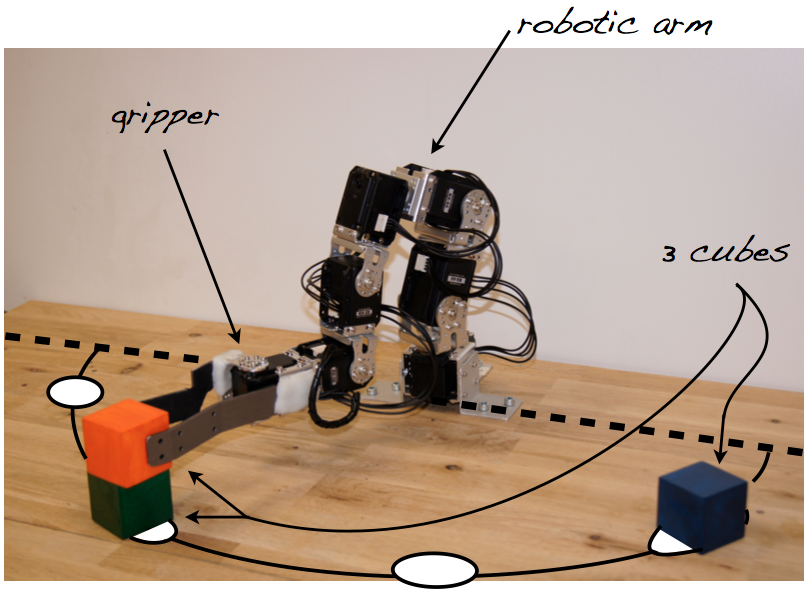
\includegraphics[width=0.49\columnwidth]{chapters/lfui/img/setup.png}
  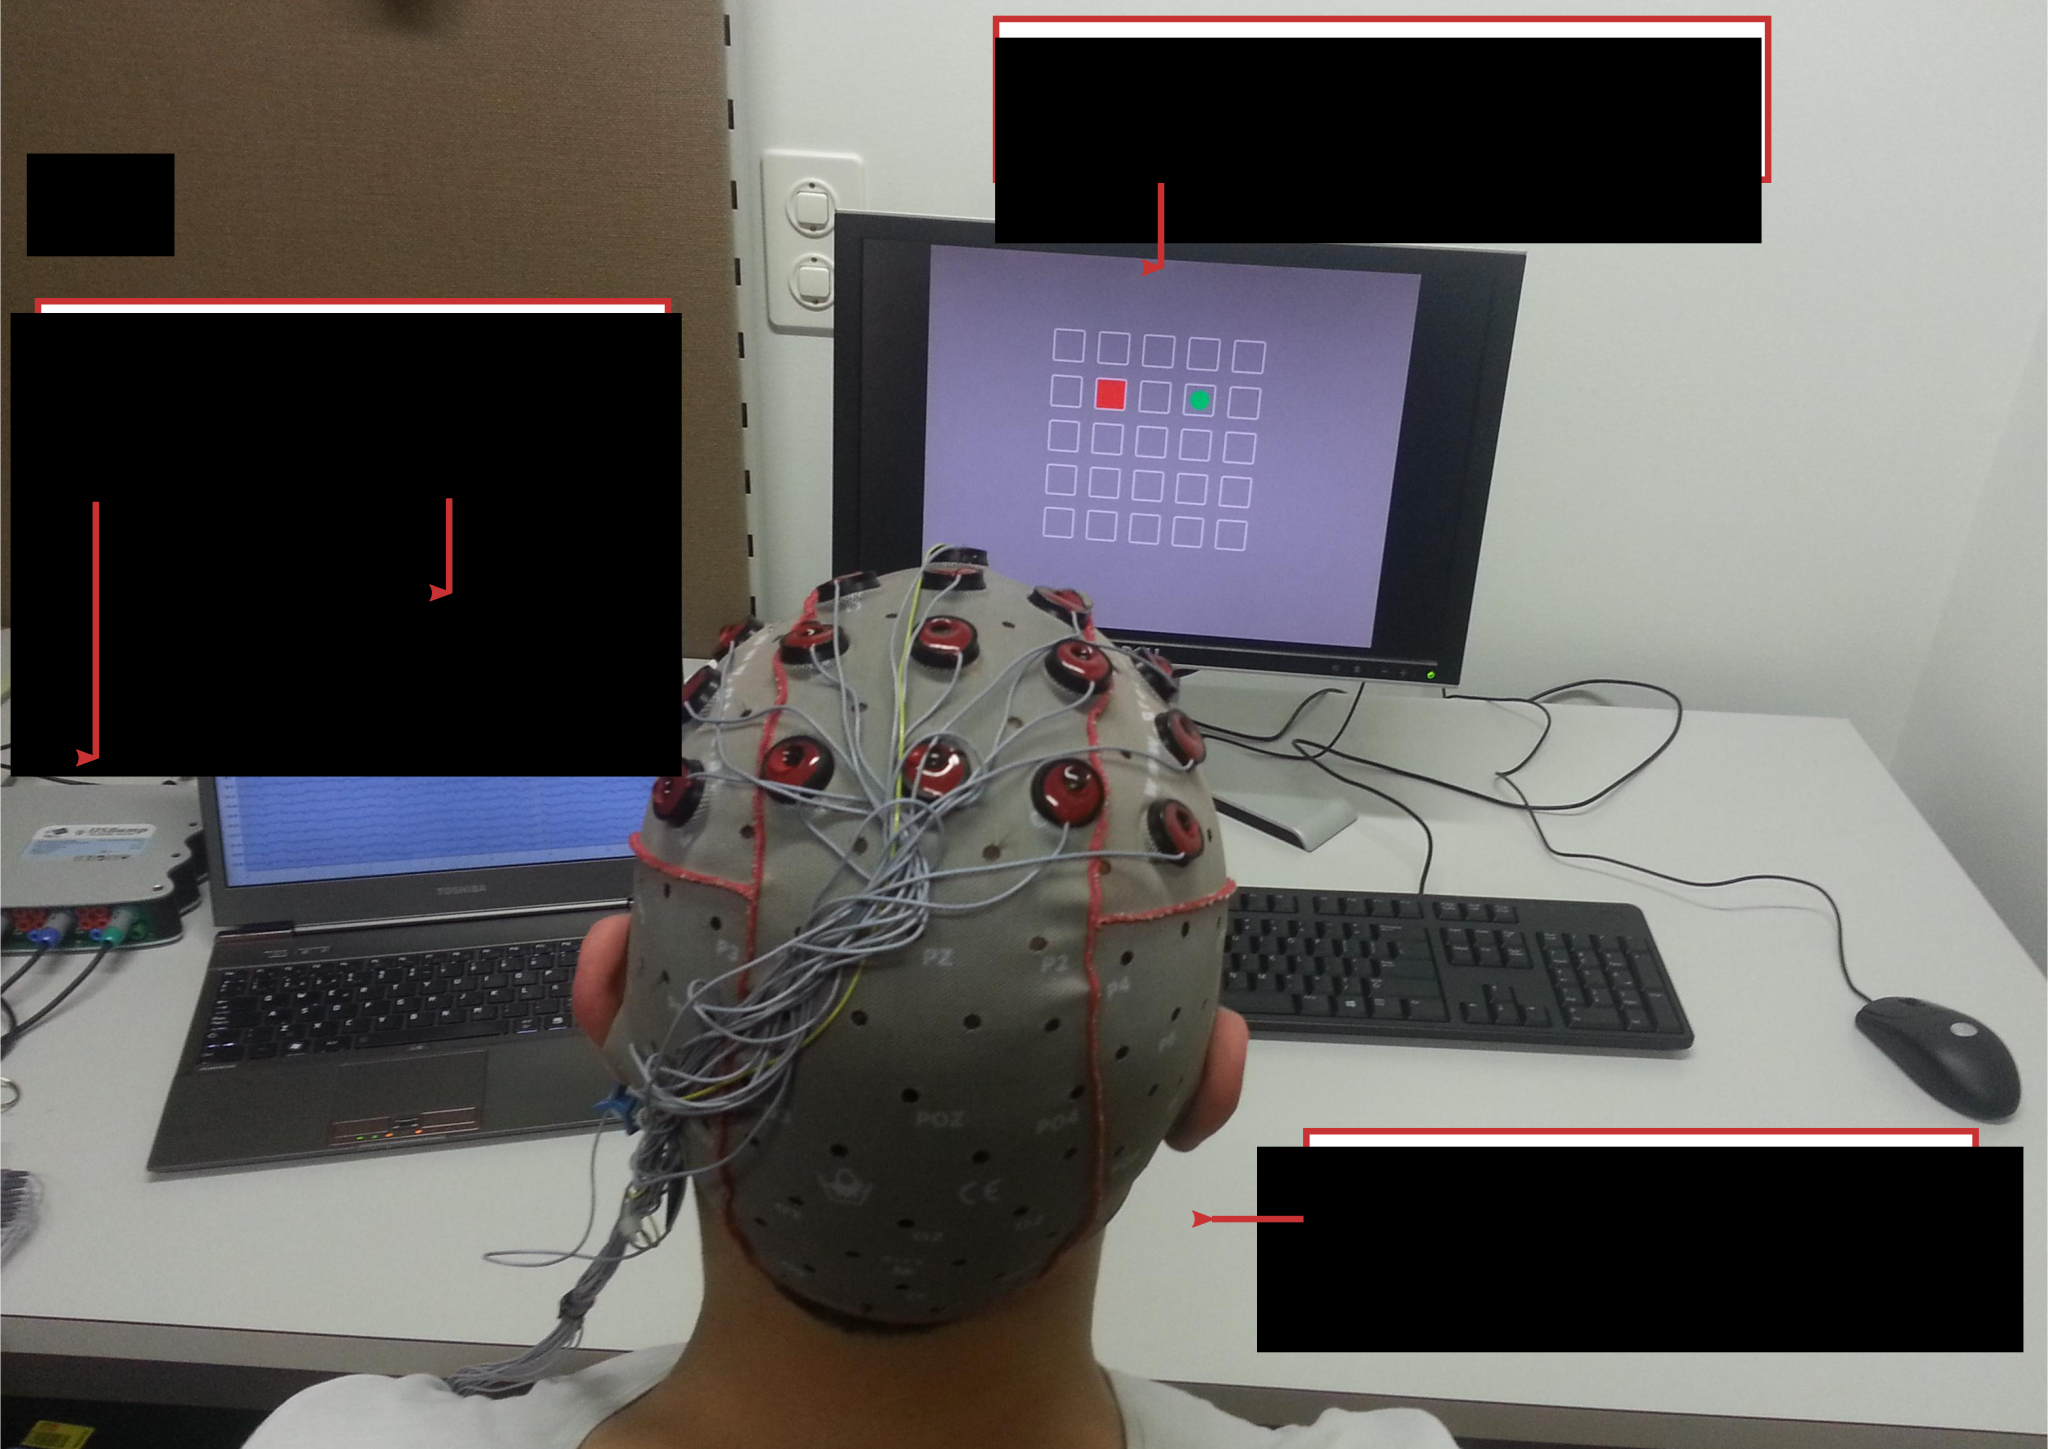
\includegraphics[width=0.49\columnwidth]{\visualspdf/onlineXP/setup.pdf}
  \caption{Illustration des deux setups expérimentaux utilisés dans ce travail. A gauche : le bras robotique pour la tâche d'organisation de trois cubes. A droite : l'interface cerveau-machine composée d'un casque avec ses électrodes et d'un écran affichant les informations relatives à la tache.}
  \label{fig:setupfrench}
\end{figure}

Bien que les expériences du chapitre~\ref{chapter:lfui} soient fondatrices, nous préférons nous concentrer pour ce bref résumé sur les expériences BCI. Elles présentent un aspect plus appliqué car testées sur de vrais sujets en temps réel et sur une tâche d'actualité pour les interfaces cerveau-machine.

Au chapitre \ref{chapter:bci}, nous présentons l'application principale de ce travail aux interfaces cerveau-machine. Ce genre d'interface permet aux personnes à fort handicap d'interagir avec le monde extérieur par le biais de leur activité cérébrale. Plus précisément, nous pouvons enregistrer des variations de potentiel à la surface de leur cerveau. Ces ondes ont des propriétés différentes en fonction de l'activité mentale du sujet. Il est possible de différentier des activités motrices, ou même des signaux d'erreur de type oui/non. Le problème de ces systèmes est qu'ils ne sont pas universels et doivent être adaptés à chaque utilisateur. Cette adaptation est faite par le biais d'une phase de calibration où l'utilisateur doit répéter plusieurs centaines de fois les mêmes actions mentales. Pendant ce temps, le système est inutilisable et l'intervention d'une personne extérieure est nécessaire. Non seulement cette phase de calibration est ennuyeuse et rébarbative, mais elle doit être effectuée régulièrement car les signaux varient de jour en jour ou car la position du casque change.

% Enfin, au chapitre \ref{chapter:bci}, nous présentons les résultats d'expériences réelles dans le cadre de l'interaction cerveau-machine.

L'utilisation d'algorithmes d'auto-calibration permettrait donc une plus grande flexibilité d'utilisation de ces technologies et permettrait de les utiliser chez soi sans la supervision d'un spécialiste.

Dans cette thèse, nous présentons donc des expériences où des sujets humains ont pour tâche de guider un agent dans un labyrinthe en lui indiquant si ces actions sont ``correctes''  ou ``incorrectes'' vis-à-vis de l'objectif défini, simplement en pensant à ``correct'' ou ``incorrect''. Les ``pensées'' de l'utilisateur sont mesurées par le biais d'électrodes au contact de son cerveau. Le setup expérimental est celui présenté sur la figure~\ref{fig:setupfrench} (droite).

La figure~\ref{fig:sequencefrench} présente le résultat principale de cette thèse. Elle compare la différence entre un algorithme nécessitant une phase de calibration et les algorithmes d'auto-calibration développés dans cette thèse. Ce sont des résultats de simulation avec des données EEG réelles. Notre algorithme (figure~\ref{fig:sequencefrench} - haut) permet de résoudre une première tâche en seulement 85 itérations, bien avant que la phase de calibration ne soit complète (400 itérations étant une période typique de calibration pour ce genre de système).
Enfin, notre méthode résout une dizaine de tâches en 400 itérations, soit avant qu'un système traditionnel ne soit opérationnel.

\begin{figure}[!htbp]
\centering
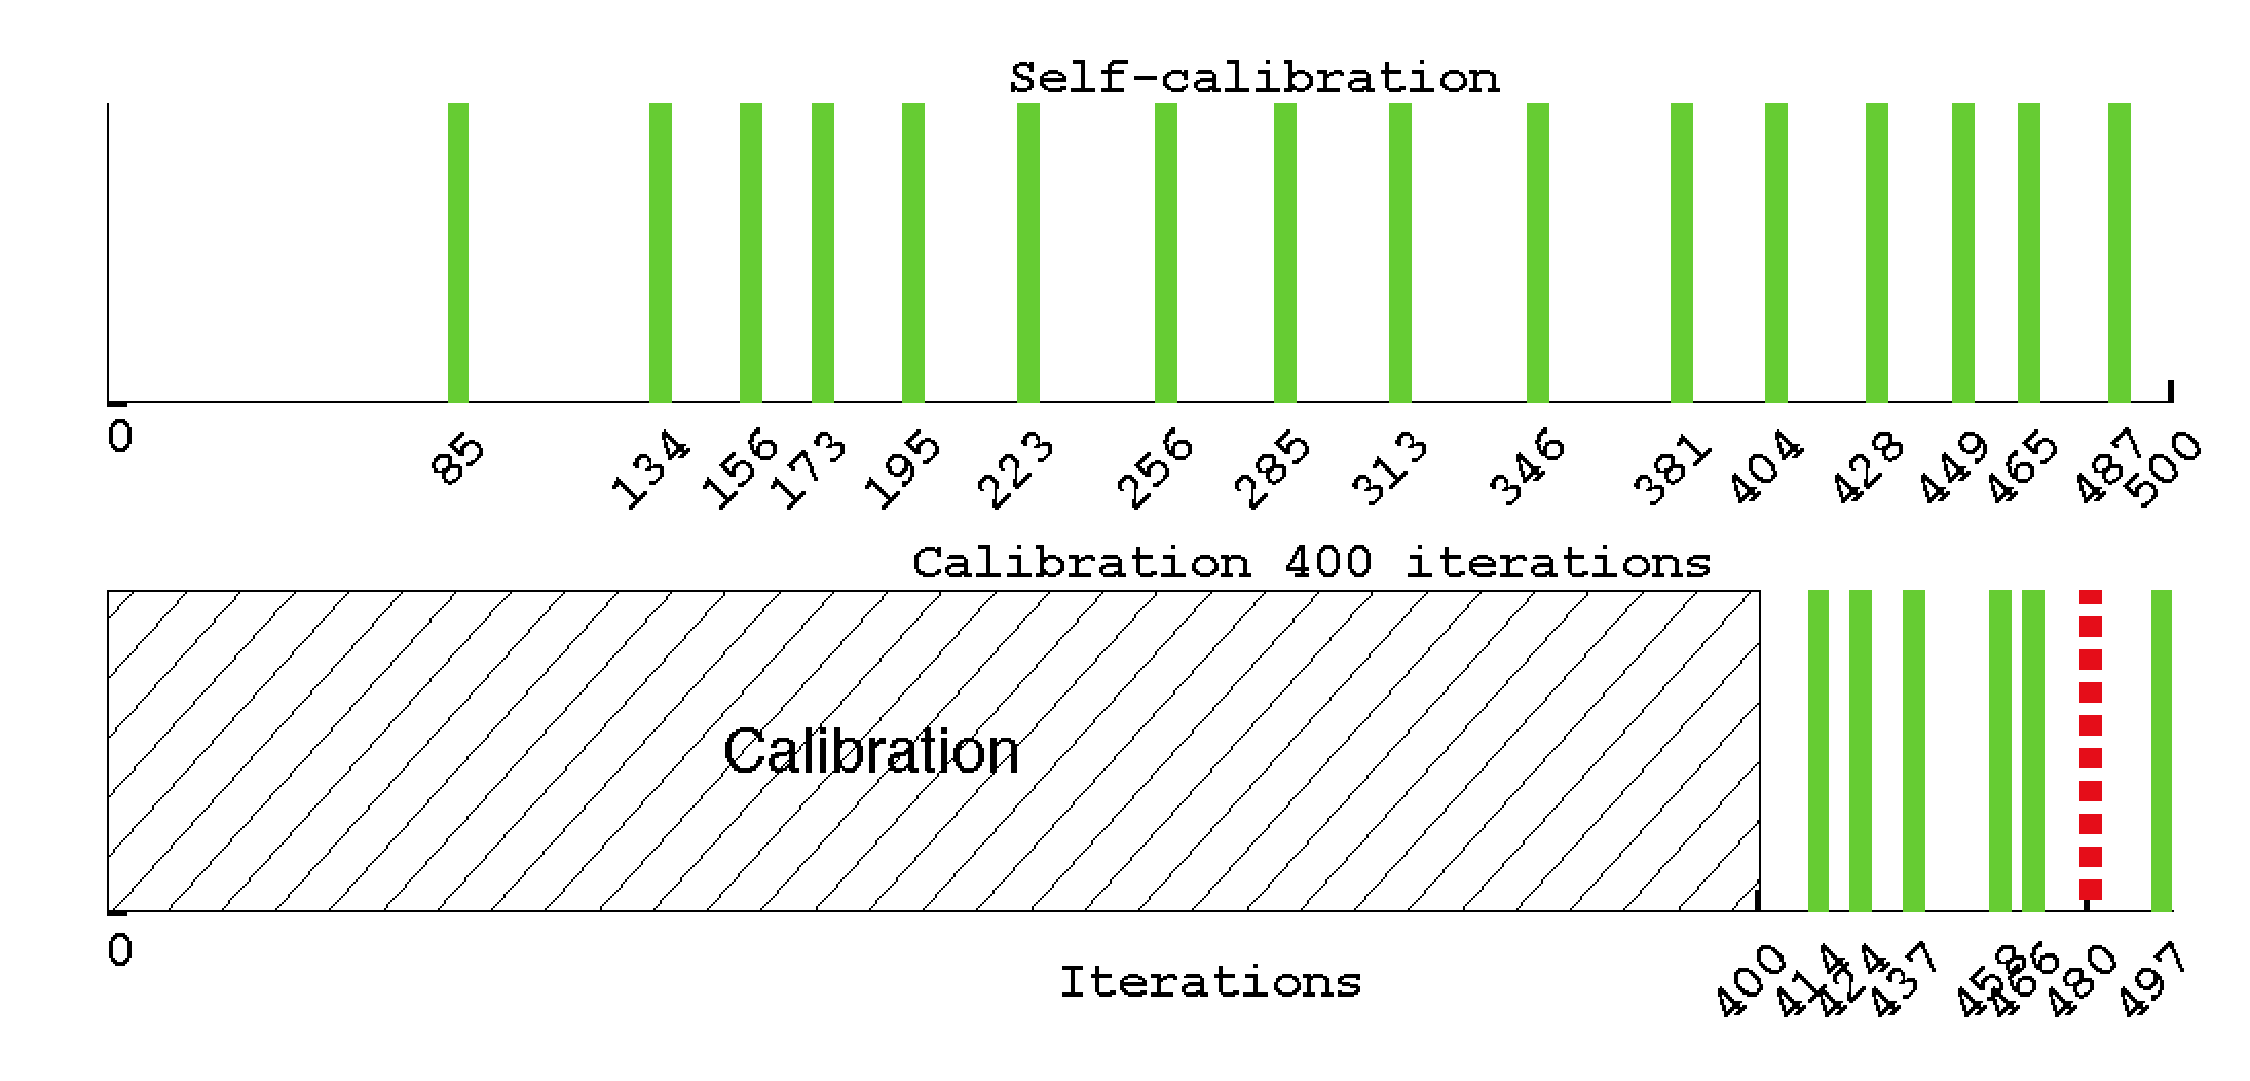
\includegraphics[width=\sequencesize\columnwidth]{\imgpath/plot_the_aaai_sequence.eps}
\caption{Nombre de tâches résolues sur 500 itérations avec des données EEG. L'algorithme d'auto-calibration (haut) est comparé aux méthodes nécessitant une phase de calibration (bas, ici 400 itérations de calibration). Les barres vertes et rouges représentent respectivement les bonnes et les mauvaises exécutions de la tâche par la machine. La méthode d’auto-calibration proposée dans cette thèse permet de compléter une première tâche plus rapidement, sans pour autant faire d'erreur.}
\label{fig:sequencefrench}
\end{figure}

Les mêmes expériences ont été faites avec des utilisateurs réels. Leurs résultats confirment ceux des simulations et sont présentés au chapitre \ref{chapter:bci} et \ref{chapter:limitations:overlap}. Nos résultats démontrent expérimentalement que notre approche est fonctionnelle et permet une utilisation pratique de l'interface plus rapidement. De plus, notre système ne nécessite pas la présence d'une personne extérieure pour se calibrer et est donc un candidat potentiel pour amener l'utilisation des interfaces cerveau-machine dans les foyers.

\subsubsection*{Planification des actions}

Les actions de la machine font partie intégrante de la performance de nos algorithmes. En effet, si la machine ne bouge pas, alors aucun signal ne sera reçu et ni la tâche ni le modèle de langage ne seront jamais appris. Nous avons donc étudié quelle stratégie de sélection des actions devrait suivre la machine afin d'apprendre le plus efficacement possible. Un certain nombre de méthodes sur des problèmes généraux exsitent. Elles consistent en général à mesurer l'incertitude sur le problème et à trouver les actions ayant la plus grande probabilité de réduire cette incertitude.

Comparé aux algorithmes existants, notre problème inclut une couche d'incertitude supplémentaire : non seulement la tâche est inconnue, mais aussi le sens des signaux. Il faut donc inclure cette double incertitude pour naviguer plus efficacement dans l'environnement et collecter des informations d'une façon optimisée. Les résultats présentés au chapitre~\ref{chapter:planning} montrent que notre méthode de planification des actions améliore significativement le temps nécessaire à l'identification de la tâche, mais aussi à l'établissement du modèle de langage de l'utilisateur.

\subsubsection*{Extensions}

Au chapitre~\ref{chapter:limitations}, nous proposons des solutions aux multiples limitations de l'approche présentée dans cette thèse. Nous montrons d'abord qu'il est possible d'utiliser nos algorithmes dans des espaces continus : premièrement pour un état continu du système (chapitre~\ref{chapter:limitations:continousstate}), mais aussi pour un ensemble infini d'hypothèses sur la tâche (chapitre~\ref{chapter:limitations:continuoushypothesis}). Par la suite, nous montrons que la connaissance a priori du protocole d'interaction n'est pas une limitation forte et que notre système peut détecter le protocole par l'interaction pratique avec l'utilisateur (chapitre~\ref{chapter:limitations:framehypothesis}).

Paradoxalement, cette thèse ne traite pas directement du problème simple et symbolique, mais s'intéresse d'abord à une représentation continue des signaux de communication. Ceci est fait dans un but applicatif, auquel de fastidieuses preuves mathématiques dans des domaines trop simplifiés n’auraient guère laissé de temps à l'expérimentation. Ainsi, la formulation simple du labyrinthe présentée au début de ce résumé n'est adressée que dans la toute dernière section de cette thèse (chapitre~\ref{chapter:limitations:proof}) par une preuve de la validité de notre solution, pour le cas de signaux de communication symboliques et sous de fortes contraintes environnementales. Ce dernier développement montre que ce genre de problème peut être modélisé mathématiquement et ouvre la voie à de prochaines explorations plus théoriques. Elles permettront peut-être d’avoir de plus grandes garanties sur la convergence et les performances de nos algorithmes. Il est à noter que ce type de preuve est encore très limité pour l'interaction pratique du fait de l’imprévisibilité du comportement humain.

% Finalement, nous démontrons mathématiquement sur un exemple simplifié et sous certaines conditions que notre méthode garantit l’identification de la bonne hypothèse.

\subsection*{Expèrience humain-humain}

Cette thèse traite également de la mise en place d'un protocole expérimental pour analyser le comportement de deux humains mis dans la situation que doivent résoudre nos algorithmes (chapitre~\ref{chapter:humanexperiment}). Dans cette expérience, deux personnes doivent collaborer à l'exécution d'une tâche de construction. Elles ne peuvent interagir que par le biais d'une interface dont le sens des signaux transmis est inconnu et indéfini au départ pour les deux parties.

Il sera intéressant de voir la dynamique de construction d'un langage commun entre les deux participants. Ce langage, qui n'était pas prévu au début de l'interaction, s'établit de telle sorte qu'une personne extérieure à l'expérience ne pourra alors pas comprendre ce qui se passe en observant le résultat final de l'interaction.

\subsection*{Conclusion}

La vision développée dans cette thèse est qu'il est possible pour une machine d'interagir avec un humain sans comprendre initialement la façon dont l'utilisateur communique. Plus concrètement, notre système n'a pas de préjugé sur le sens des signaux reçus et construit son modèle durant l'interaction pratique avec l'utilisateur sans jamais avoir accès à une source sûre d'information. Nous espérons que cela sera le fruit de nombreux travaux futurs.

Au-delà du défi technique de l'auto-calibration, des questions pratiques d'utilisation et d'acceptabilité apparaissent et sont présentées au chapitre~\ref{chapter:limitations:userstudies}. La plus importante à tester en condition réelle est la réaction qu’auront les utilisateurs face au fait que la machine, i.e. le robot, ne soit pas immédiatement réactif à leurs ordres. Le robot doit en effet apprendre le sens des signaux pendant l'interaction. Même si nos algorithmes apportent une plus grande flexibilité d'interaction, ils ne permettent pas à l'utilisateur une fonctionnalité immédiate et parfaite du système. Cette phase d'apprentissage pourrait être perçue comme une déficience et par conséquent impacter l'intérêt et l'utilisabilité réelle de notre système.\\

\noindent {\large\textbf{Mots-clés :}} Auto-Calibration, Apprentissage par Interaction, Interaction Humain-Robot, Interface Cerveau-Machine, Interaction Intuitive et Adaptative, Robotique, Acquisition de Symboles, Apprentissage Actif, Calibration.\\

Ce travail a été financé par INRIA, le Conseil Régional d'Aquitaine et la bourse ERC EXPLORERS 24007.
